\subsection{Electric Networks}
\label{ssec:electric-networks}

The final presented application comes from engineering. In
\myref{figure}{fig:car-circuit}, you can see a simplified version of a car's
electric network.

\begin{figure}[ht]
 \centering
 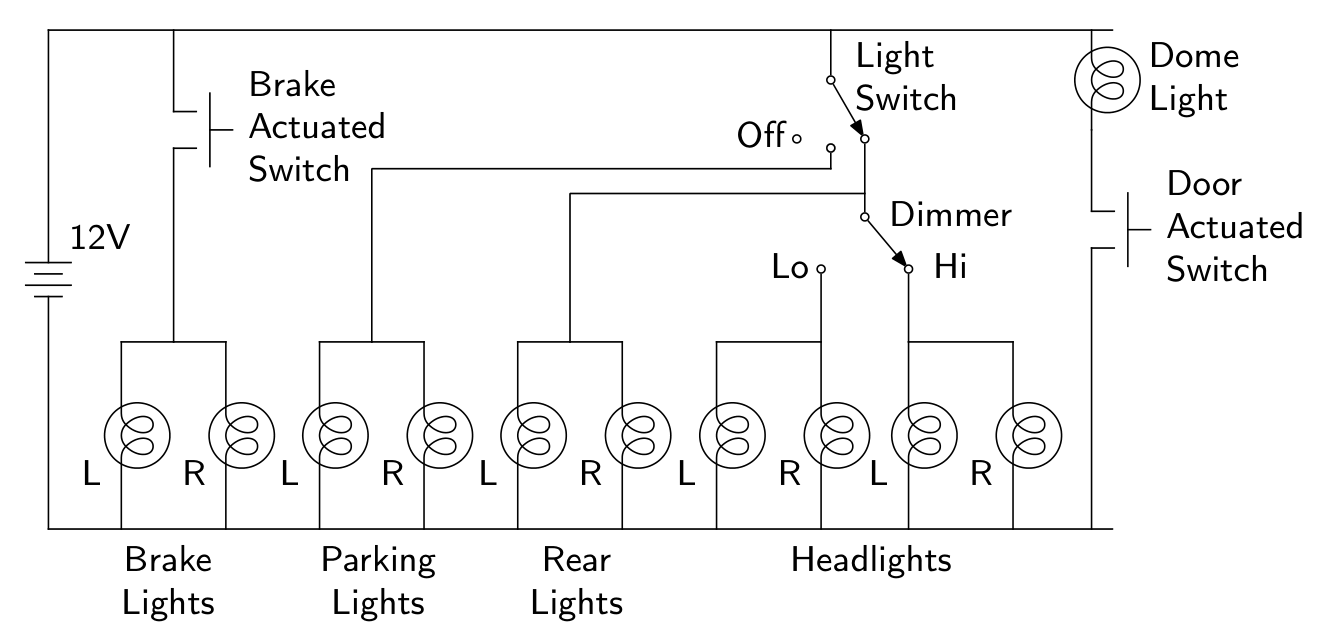
\includegraphics[width=.8\textwidth]{figs/car-circuit}
 \caption{An excerpt from a car's electric network.}
 \label{fig:car-circuit}
\end{figure}

A designer of this network must be able to answer questions similar to: `How
much electricity flows when both the hi-beam headlights and the brake lights are
on?' Even very sophisticated electric networks can be analysed using Kirchhoff's
laws and the theory of linear systems.

The intuitive explanation of electric circuits (which suffices for our purposes)
tells that there are three interconnected forces at play -- voltage $(U)$,
resistance ($R$) and current ($I$). At any point of the circuit, these are tied
by the formula $U = RI$. The battery serves as a capacitor; it provides
\emph{voltage} -- or electric potential -- to the circuit, making electricity
flow as long as there is a path. The moment a path is formed (we say the circuit
is closed), the battery creates a force through the circuit -- the
\emph{current}. Finally, some components of the circuit act as \emph{resistors},
effectively limiting the amount of voltage that is `available' to the subsequent
components of the circuit. This limiting factor is the \emph{resistance} of the
component and is often proportional to the force provided by the battery. We can
think of the resistors causing \emph{voltage drops} throughout the current
whilst the battery provides a \emph{voltage rise}.

To interpret electric networks (basically meshes of electric circuits) as linear
systems, two physical laws are needed -- \emph{Kirchhoff's Current Law} and
\emph{Kirchhoff's Voltage Law}. The former states that at any point in the
network, the flow in equals the flow out. The latter then that around any
circuit in the network, the total voltage rise equals the total voltage drop.

Let us start with a simple network consisting of a single circuit.
\begin{figure}[ht]
 \centering
 \begin{circuitikz}
  \draw (0,0) to [R, l^=$3 \Omega$] (5,0)
        (5,0) to [R, l^=$5 \Omega$] (5,3)
        (5,3) to [R, l^=$2 \Omega$] (0,3)
        (0,3) to [battery, l^=$20 V$] (0,0);
 \end{circuitikz}
 \caption{An electric circuit with a battery and three resistors.}
 \label{fig:electric-network-1}
\end{figure}

The component represented by~\tikz[baseline=.1cm,scale=0.4, every
node/.style={scale=0.4}]{\draw (0,0) to [battery] (0,1);} is the battery
and~\tikz[baseline=-.1cm,scale=0.4, every node/.style={scale=0.4}]{\draw (0,0)
to [R] (1,0);} depicts a resistor. We measure voltage provided by the battery in
\emph{volts} ($V$) and the resistance of the other components in \emph{ohms}
($\Omega$).

Since this network features only a single closed circuit, the current --
measured in \emph{amperes} ($A$) -- is consistent throughout by Kirchhoff's
Current Law. By Kirchhoff's Voltage Law, the total voltage rise (which is $20
V$) equals the total voltage drop. In this circuit, there are three voltage
drops, each equal to the resistance of the component times the current flowing
through it. This gives us a linear system consisting of the single equation
\[
 20 = 2I + 5I + 3I
\]
wherefrom we infer that $I = 2 A$; the current around the circuit equals $2$
amperes.

An example of a network leading to a more elaborate linear system requires
connecting the resistors \emph{in parallel} which automatically creates more
circuits in the network.
\begin{figure}[ht]
 \centering
 \begin{circuitikz}[scale=0.75]
  \draw (0,0) to (7,0)
        (7,0) to (7,1)
        (7,1) to (5,1)
        (5,1) to [R,l^=$12 \Omega$] (5,4)
        (7,1) to (9,1)
        (9,1) to [R,l_=$8 \Omega$] (9,4)
        (5,4) to (7,4)
        (9,4) to (7,4)
        (7,4) to (7,5)
        (7,5) to (0,5)
        (0,5) to [battery,l^=$20 V$] (0,0);
  \draw[-latex,thick] (2,4.7) to node[below] {$i_0$} (5,4.7);
  \draw[-latex,thick] (5.5,3.5) to node[right] {$i_1$} (5.5,1.5);
  \draw[-latex,thick] (8.5,3.5) to node[left] {$i_2$} (8.5,1.5);
 \end{circuitikz}
 \caption{An electric network with resistors connected in parallel.}
 \label{fig:electric-network-2}
\end{figure}

It might not look like it but the network in
\myref{figure}{fig:electric-network-2} actually hosts three circuits depicted in
\myref{figure}{fig:electric-network-3}.
\begin{figure}[ht]
 \centering
 \begin{subfigure}[b]{.3\textwidth}
  \centering
  \begin{circuitikz}[scale=0.3,every node/.style={scale=0.5}]
   \draw[thick,BrickRed]
        (0,0) to (7,0)
        (7,0) to (7,1)
        (7,1) to (5,1)
        (5,1) to [R] (5,4);
   \draw
        (7,1) to (9,1)
        (9,1) to [R] (9,4)
        (9,4) to (7,4);
   \draw[thick,BrickRed]
        (5,4) to (7,4)
        (7,4) to (7,5)
        (7,5) to (0,5)
        (0,5) to [battery] (0,0);
  \end{circuitikz}
  \caption{First \clr{circuit}.}
 \end{subfigure}
 \begin{subfigure}[b]{.3\textwidth}
  \centering
  \begin{circuitikz}[scale=0.3,every node/.style={scale=0.5}]
   \draw[thick,RoyalBlue]
        (0,0) to (7,0)
        (7,0) to (7,1)
        (7,1) to (9,1)
        (7,5) to (0,5)
        (0,5) to [battery] (0,0)
        (9,1) to [R] (9,4)
        (9,4) to (7,4)
        (7,4) to (7,5);
   \draw
        (5,4) to (7,4)
        (7,1) to (5,1)
        (5,1) to [R] (5,4);
  \end{circuitikz}
  \caption{Second \clb{circuit}.}
 \end{subfigure}
 \begin{subfigure}[b]{.3\textwidth}
  \centering
  \begin{circuitikz}[scale=0.3,every node/.style={scale=0.5}]
   \draw[thick,ForestGreen]
        (7,1) to (9,1)
        (9,1) to [R] (9,4)
        (5,1) to [R] (5,4)
        (5,4) to (7,4)
        (9,4) to (7,4)
        (7,1) to (5,1);
   \draw
        (7,4) to (7,5)
        (7,5) to (0,5)
        (0,5) to [battery] (0,0)
        (7,0) to (7,1)
        (0,0) to (7,0);
  \end{circuitikz}
  \caption{Third \clg{circuit}.}
 \end{subfigure}
 \caption{The three circuits of an electric network.}
 \label{fig:electric-network-3}
\end{figure}
Each of those circuits obeys Kirchhoff's Voltage Law. Spelt out for the
\clr{first circuit}, it says the total voltage rise of $20 V$ must equal the
total voltage drop of $12 \Omega$ times the current flowing through this
circuit, which we labelled $i_1$. Similarly, the voltage rise in the \clb{second
circuit} is $20 V$ and equals $8i_2$. Finally, the voltage rise in \clg{circuit
three} is $0 V$ and equals the voltage drop through the first resistor plus the
voltage drop through the second resistor. The only caveat here is the choice of
orientation of the current. The current flowing through the first resistor must
do so in direction opposite to the second resistor as the circuit forms a closed
oriented loop. This means that one of the currents (for instance $i_2$) must be
given a negative sign, signifying a direction of flow opposite to the one in
\clb{circuit two}. This gives a total voltage drop in the \clg{third circuit} as
$12i_1 - 8i_2$.

Finally, there are two points in the network where the flow splits. Applying
Kirchhoff's Current Law thus awards two more equations: $i_0 = i_1 + i_2$ and
$i_1 + i_2 = i_0$. All in all, we ended up with a linear system of five
equations.
\begin{equation}
 \label{eq:electric-network-2}
 \begin{array}{r c r c r c r}
  & & 12i_1 & & & = & 20\\
  & & & & 8i_2 & = & 20\\
  & & 12i_1 & - & 8i_2 & = & 0\\
  i_0 & - & i_1 & - & i_2 & = & 0\\
  -i_0 & + & i_1 & + & i_2 & = & 0
 \end{array}
\end{equation}
Clearly, there are redundant equations in the
system~\eqref{eq:electric-network-2}. This just goes to show that redundancy
arises in practice and the problem of determining which equations are redundant
is generally not entirely trivial; we shall discuss it later in the book.

In this case, of course, the first two equations already give us equalities $i_1
= \frac{5}{3}A$ and $i_2 = \frac{5}{2}A$. Finally, the fourth equation (or the
fifth for that matter) ensures that $i_0 = \frac{25}{6} A$. Hence, the total
current through the entire network is $\frac{25}{6} A$.

The final example to discuss is the so-called
\href{https://en.wikipedia.org/wiki/Wheatstone_bridge}{Wheatstone Bridge}.
\begin{figure}[ht]
 \centering
 \begin{circuitikz}[scale=0.75,every node/.style={scale=0.75}]
  \draw
   (0,0) to (8,0)
   (8,0) to (8,1)
   (8,1) to [R,l^=$10 \Omega$] (5,3)
   (5,3) to [R,l^=$5 \Omega$] (8,5)
   (8,1) to [R,l_=$4 \Omega$] (11,3)
   (11,3) to [R,l_=$2 \Omega$] (8,5)
   (5,3) to [R,l_=$50 \Omega$] (11,3)
   (8,5) to (8,6)
   (8,6) to (0,6)
   (0,6) to [battery,l_=$10 V$] (0,0);
 \end{circuitikz}
 \caption{The \href{https://en.wikipedia.org/wiki/Wheatstone_bridge}{Wheatstone
 Bridge} network.}
 \label{fig:wheatstone-bridge}
\end{figure}
There is \emph{a lot} of circuits in this network. We first choose an arbitrary
orientation of the currents through each of the branches as in
\myref{figure}{fig:wheatstone-bridge-2}.
\begin{figure}[ht]
 \centering
 \begin{circuitikz}[scale=0.5,every node/.style={scale=0.5}]
  \draw
   (0,0) to (8,0)
   (8,0) to (8,1)
   (8,1) to [R] (5,3)
   (5,3) to [R] (8,5)
   (8,1) to [R] (11,3)
   (11,3) to [R] (8,5)
   (5,3) to [R] (11,3)
   (8,5) to (8,6)
   (8,6) to (0,6)
   (0,6) to [battery] (0,0);
  \draw[thick,-latex] (2,5.7) to node[below] {\huge $i_0$} (6,5.7);
  \draw[thick,-latex,shorten <=5pt,shorten >=5pt] (7.7,5.3) to node[above left]
  {\huge $i_1$} (4.7,3.3);
  \draw[thick,-latex,shorten <=5pt,shorten >=5pt] (8.3,5.3) to node[above right]
  {\huge $i_2$} (11.3,3.3);
  \draw[thick,-latex,shorten <=5pt,shorten >=5pt] (4.7,2.7) to node[below left]
  {\huge $i_3$} (7.7,0.7);
  \draw[thick,-latex,shorten <=5pt,shorten >=5pt] (11.3,2.7) to node[below
  right] {\huge $i_4$} (8.3,0.7);
  \draw[thick,-latex,shorten <=8mm,shorten >=8mm,yshift=5mm] (5,3) to
  node[above] {\huge $i_5$} (11,3);
  \draw[thick,-latex] (6,0.3) to node[above] {\huge $i_0$} (2,0.3);
 \end{circuitikz}
 \caption{A choice of current orientation in the
 \href{https://en.wikipedia.org/wiki/Wheatstone_bridge}{Wheatstone Bridge}
network.}
 \label{fig:wheatstone-bridge-2}
\end{figure}

We can't yet be sure how many or which equations we will need to calculate $i_0$
-- the total current. We definitely need at least 6 given the number of
variables. Kirchhoff's Current Law yields many equations but we (based mostly on
intuition) pick these three:
\[
 \begin{array}{r c r c r}
  i_0 & = & i_1 & + & i_2\\
  i_3 & + & i_4 & = & i_0\\
  i_2 & + & i_5 & = & i_4
 \end{array}
\]
We've chosen these particular equations in a way that makes every variable
appear at least once. Using Kirchhoff's Voltage Law on the inner, outer and the
upper `triangle-shaped' circuit gives respectively:
\[
 \begin{array}{r c r c r c r}
  10 & = & 5i_1 & + & 10i_3 & & \\
  10 & = & 2i_2 & + & 4i_4 & & \\
  0 & = & 5i_1 & + & 50i_5 & - & 2i_2
 \end{array}
\]
Again, we have chosen these equations in order to make the resistance of every
component appear at least once. Having collected the six equations into a linear
system, we pray that we get a unique solution.
\[
 \begin{array}{r c r c r c r c r c r c r}
  i_0 & - & i_1 & - & i_2 & & & & & & & = & 0\\
  -i_0 & & & & & + & i_3 & + & i_4 & & & = & 0\\
       & & & & i_2 & & & - & i_4 & + & i_5 & = & 0\\
       & & 5i_1 & & & + & 10i_3 & & & & & = & 10\\
       & & & & 2i_2 & & & + & 4i_4 & & & = & 10\\
       & & 5i_1 & - & 2i_2 & & & & & + & 50i_5 & = & 0
 \end{array}
\]
And\dots~yes! We do. As SageMath confirms.
\begin{Verbatim}
sage: A = \clb{Matrix}(QQ, [
....:     [\clr{1}, \clr{-1}, \clr{-1}, \clr{0}, \clr{0}, \clr{0}],
....:     [\clr{-1}, \clr{0}, \clr{0}, \clr{1}, \clr{1}, \clr{0}],
....:     [\clr{0}, \clr{0}, \clr{1}, \clr{0}, \clr{-1}, \clr{1}],
....:     [\clr{0}, \clr{5}, \clr{0}, \clr{10}, \clr{0}, \clr{0}],
....:     [\clr{0}, \clr{0}, \clr{2}, \clr{0}, \clr{4}, \clr{0}],
....:     [\clr{0}, \clr{5}, \clr{-2}, \clr{0}, \clr{0}, \clr{50}],
....: ])
sage: b = \clb{vector}(QQ, [\clr{0}, \clr{0}, \clr{0}, \clr{10}, \clr{10}, \clr{0}])
sage: A.\clm{solve_right}(b)
(\clr{7/3}, \clr{2/3}, \clr{5/3}, \clr{2/3}, \clr{5/3}, \clr{0})
\end{Verbatim}
A somewhat surprising fact about this solution is the equality $i_5 = 0$,
meaning no electricity flows through the corresponding component.

\begin{exercise}{}{electric-network}
 \myref{Figure}{fig:electric-network-4} depicts an electric network.
 \begin{figure}[H]
  \centering
  \begin{circuitikz}
   \draw
    (0,0) to (3,0)
    (3,0) to [R,l^=$2 \Omega$] (6,0)
    (3,0) to [R,l_=$3 \Omega$] (3,2)
    (6,0) to [R,l^=$2 \Omega$] (9,0)
    (6,0) to [R,l^=$2 \Omega$] (6,2)
    (9,0) to [R,l^=$4 \Omega$] (9,2)
    (3,2) to [R,l_=$3 \Omega$] (6,2)
    (6,2) to [R,l_=$3 \Omega$] (9,2)
    (0,2) to (3,2)
    (0,0) to [battery,l_=$9 V$] (0,2);
  \end{circuitikz}
  \caption{An electric network with 7 resistors.}
  \label{fig:electric-network-4}
 \end{figure}
 Calculate the current in each branch of the network.
\end{exercise}
